
\clearpage
\section{Bottleneck clarification and scan comparison (13 October update)}
\label{sec:bottleneck}
\textbf{The current model is limited first by total CPU demand, then by online
communication. Storage is large, but is not the binding constraint at the selected
point.} This is a diagnosis of the analytical model, not a measured profile of an
implemented MPC service. The earlier report combined online and preprocessing
work; the new ledger separates them without changing its total costs.

For the selected 128-query batch on six \texttt{r6in.24xlarge} machines per party:
\begin{center}\begin{tabular}{lr}\toprule
Resource or dependency & Time per batch\\\midrule
CPU, including preprocessing & 3.452 s\\
Network, including preprocessing and internal routing & 2.225 s\\
Modeled RAM traffic & 0.094 s\\
Dependent exchanges & 1.291 s\\\midrule
Service time: $1.291+\max(3.452,2.225,0.094)$ & 4.743 s\\
\bottomrule\end{tabular}\end{center}
These resource times are not additive under the model's overlap assumption.
Total mean response time is about 4.77 s after batch formation and fixed response
overhead. Faster CPUs eventually make networking or round latency dominant.

\subsection{What is offline and what is online?}
The selected SY-Shamir backend does not consume one Beaver triple per scalar
multiplication. Its main product/degree-reduction traffic depends on the live
inputs. Preprocessing supplies fresh checking randomness, random bits, and
canonical masks. Thus importing a triple-generation bottleneck from a different
SPDZ backend would misdiagnose this model.

\begin{center}\begin{tabular}{lrrr}\toprule
Per party, per logical read & Preprocessing & Online & Total\\\midrule
Sent traffic, decimal MB & 148.0 & 481.1 & 629.2\\
CPU proxy, million weighted operations & 122.9 & 216.9 & 339.8\\
\bottomrule\end{tabular}\end{center}
The traffic includes 5\% framing, counts each send once, and excludes intraparty
redistribution. CPU units are weighted source-operation estimates, not measured
cycles or seconds. All ten parties incur the corresponding resource demand.

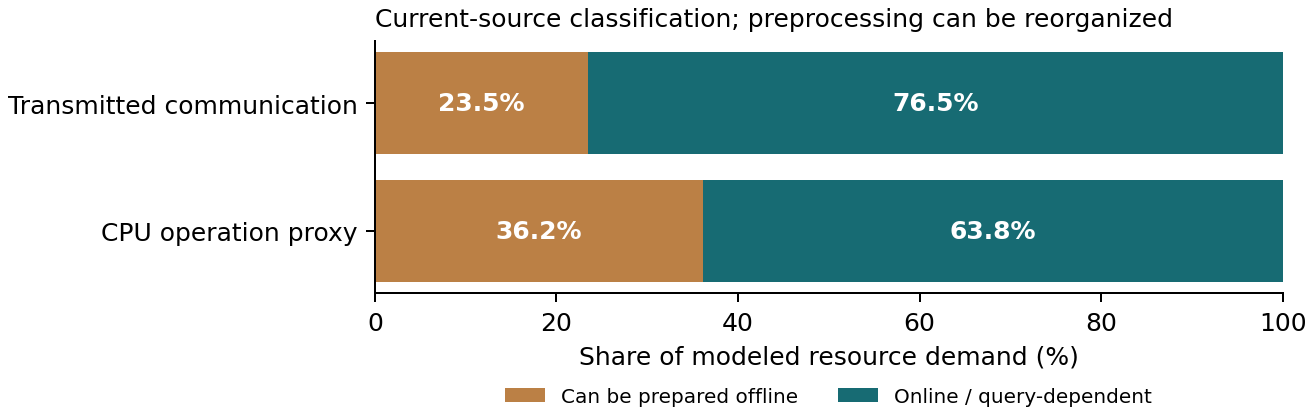
\includegraphics[width=\linewidth]{results/online_offline_breakdown.png}

For $O$ scalar/dot outputs, $C$ canonical masks, and $B_r$ random bits, the leading
preprocessing allocation is
\begin{align*}
 W_{\rm off}&=\tfrac56O+9(126C)+24B_r+8C,\\
 A_{\rm off}&=15O+68(126C)+330B_r+35C.
\end{align*}
$W$ counts transmitted field words per party; $A$ is the local CPU proxy. A full
output costs $9+5/6$ words: 9 for query-dependent resharing and 5/6 for a fresh secret
checking coefficient. Mask acceptance uses 126 outputs and an opening offline.
Fixed checks add small terms retained in the program. The online column is the
unchanged total minus this allocation.\footnote{Source accounting is pinned to
MP-SPDZ commit \texttt{73eb8556cdfc670c5d3dc1067a3ae5b4ad0d4441}; see
\url{https://github.com/data61/MP-SPDZ/tree/73eb8556cdfc670c5d3dc1067a3ae5b4ad0d4441/Protocols}
and the local ledger \texttt{data/mpc\_sources.txt}. These are derived counts,
not an official benchmark table.}

\textbf{The CPU phase boundary can move.} Precomputing random polynomial
contributions to scalar resharing can shift another 48 operations per live scalar
output out of the online loop. In this sensitivity, preprocessing rises from
36.2\% to about 81.1\% of total CPU work, with unchanged steady-state arithmetic.
This requires additional material storage, memory traffic, and a correct scheduling
implementation. It does not make that computation or its dollar cost disappear.
The 9-word live communication remains query-dependent. Likewise, ready preprocessing
can improve response time even when the service's sustainable throughput is still
limited by generating it. The existing 4.74 s service estimate charges full resource
production per batch; it is not an online-only latency benchmark.

\subsection{Storage and replication}
The selected state is 1,926 GiB (1.88 TiB) per party per ORAM replica, or about 2,217 GiB
including the modeled scratch/reserve. At 75\% usable memory, each 768 GiB instance
provides 576 GiB, so four machines suffice for capacity. Six are selected to meet
the latency/throughput model. Removing the memory constraint and re-searching the
same instance size leaves the selected price unchanged. Storage would become
binding under another representation or scheduling policy; field-bit metadata
in particular expands it substantially.

The previous \$2.33B/year deployment dedicates machines to each of 530 independently
evolving ORAM states. An asynchronous scheduler could share machines across those
states during round waits. The aggregate CPU-capacity requirement is 2,312 machines
per party (about \$1.69B/year), and their aggregate RAM could hold those 530 states.
That is a resource-capacity estimate, not proof that a scheduler achieves the
latency bound. The extra dedicated-instance cost is not an inherent cryptographic
lower bound. Do not allocate VM dollars proportionally to the CPU/traffic percentages:
one fleet serves overlapping demands.

\subsection{Naive parallel full-key scan}
The direct baseline compares every query key with all $N=2^{28}$ stored keys,
then returns $\sum_i [k_i=q]v_i$. Comparisons run in parallel across rows and queries;
rows are visited in a public order. Values use three private dot products, so their
selection communicates per output, not per record. There is no ORAM maintenance.
The dictionary has unique keys; the sum of match bits gives a private hit indicator.

The baseline uses \emph{exact} equality optimized for this field.
Represent a key with the same three field limbs as the ORAM. Since
$p=2^{127}-1\equiv3\pmod4$, $-1$ is a quadratic nonresidue and
$a^2+b^2=0$ holds exactly when both inputs are zero. For limb differences $d_0,d_1,d_2$,
compute
\[
 u=d_0^2+d_1^2,\qquad v=u^2+d_2^2,\qquad e=1-v^{p-1}.
\]
Each sum of squares is a length-two private dot product with one reduced output;
the 135-product exponentiation is the addition-chain routine from the model.
Thus each comparison costs 137 secure outputs, versus 407 for independently
zero-testing and combining three limbs. This equality also improves the ORAM's
few final key checks, but changes its millions-of-outputs total by less than 0.1\%.
Intermediate dot results must be degree-reduced before reuse.

Ignoring the tiny shared frontend, the full scan requires
\[
 G_{\rm scan}=137N+3\simeq36.8\ \text{billion outputs/read}.
\]
Batching does \emph{not} divide this count by batch size: a batch has $137NB$
comparison outputs. It reduces communication scheduling overhead and permits
database-cache reuse. Use row/query tiling, not an $N\times B$ materialized equality
matrix. The read-only 48 GiB of authenticated database shares per party can be shared
across concurrent workers, unlike independent mutable ORAM placements.

\subsection{An indexed alternative using private dot products}
An indexed scan is another baseline: keep the same two cuckoo tables
and scan their arrays without ORAM. Private dot products allow a two-dimensional
read. Arrange each $D=2^{29}$-cell table as an $A\times C$ matrix, with $AC=D$.
For private row and column one-hot vectors $a,b$, compute, for each payload word,
\[
 z_i=\sum_j b_jX_{ij},\qquad y=\sum_i a_i z_i.
\]
This reads every cell through local arithmetic, but only $AW+W$ dot outputs are
reduced. With $W=6$ key/value words, communication is minimized near
$A=\sqrt{D/(W+1)}$. The model chooses $A=8192,C=65536$. One-hot generation is charged,
both tables are always probed, and full keys plus the cuckoo stash are checked
exactly. Empty-cell validity can use an unused bit in the last key limb, so the
six-word payload need not grow. This is a derived exact read construction; it
does not imply a fast write protocol.

Its approximately 249,000 outputs/read are \emph{fewer} than the ORAM reference,
but its dot products still process both full arrays. The current source proxy
charges approximately $4\cdot2DW=25.77$ billion local operations/read before the
small remaining costs. Packing the batch as matrix multiplication can change
the actual cycles/operation; this must be measured independently. Our CPU-rate
assumption is not a benchmark of that dense kernel. Both scan variants can pipeline
queries and reuse immutable shares without paying for one full state per worker.

\subsection{Side-by-side work and cost}
\begin{center}\small\begin{tabular}{lrrr}\toprule
Per logical read / party & OPRAM & Full-key scan & Indexed 2D scan\\\midrule
Secure outputs & 3.36M & 36.78B & 0.249M\\
Local CPU proxy & 0.340B & 3,059B & 25.79B\\
Sent bytes, including framing & 629MB & 6.08TB & 41.2MB\\
Persistent shares & 1,926GiB & 48GiB & 192GiB\\
Exchange-depth contribution & 1.291s & 0.030s & 0.031s\\\bottomrule
\end{tabular}\end{center}
Storage is per complete state per party, not per read. Exchange-depth figures
are only the phase-delay term at 0.2 ms/exchange; they are not achievable response
latencies without sufficient computation and networking. Memory traffic is
optimistically tiled/reused for scans; detailed scratch and reduction aggregation
are not claimed to be free in an implementation.

Under the \emph{same unmeasured} 2-billion-weighted-operations/s per 64-vCPU assumption,
the common aggregate resource-capacity calculation gives:
\begin{center}\begin{tabular}{lr}\toprule
Construction & Annual resource equivalent, ten parties\\\midrule
OPRAM reference & \$1.69 billion\\
Naive full-key scan & \$15.25 trillion\\
Indexed 2D dot scan & \$128.6 billion\\\bottomrule\end{tabular}\end{center}
These all use \texttt{r6in.24xlarge} at the same 12 October price snapshot, 70\%
distributed efficiency and 70\% utilization. They are not new deployment quotes.
The scan fleets are astronomically large extrapolations, not plausible AWS
reservations. The common calculation excludes detailed sharded-dot aggregation,
queue/SLA feasibility, setup and scratch provisioning; its purpose is to expose
the scale of work. The previous \$2.33B ORAM figure includes a particular dedicated
replica policy and should not be compared with a CPU-only scan calculation as
if both were equally complete deployments.

Relative to the OPRAM reference, the naive scan needs about 9,000 times the CPU
proxy and 9,656 times the traffic. The stronger indexed scan needs about 76 times
the CPU proxy but only 6.5\% of the traffic. Therefore ``scan is communication-heavy''
is true for the naive full-key implementation, but false as a universal statement.

\paragraph{Practical conclusion.}
The next measurements should isolate (1) total preprocessing production,
(2) live product/resharing throughput, (3) checked network exchanges and
(4) a batched local matrix-contraction kernel. The current arithmetic OPRAM
reference uses less modeled CPU work than these scans, while the two-dimensional scan is
a serious bandwidth-oriented comparator. Neither the numerical CPU split nor
the cheapest real system is settled without those measurements.

Reproduce the comparison with \texttt{python -m mpc\_cost.compare\_scans};
the complete ledger is \texttt{results/bottleneck\_scan\_comparison.json}.
